\scanpage{4}

4) \uline{Élargissage} Opération inverse -- au lieu de retrancher une couronne, on en rajoute une...

5) Opération mixte : \uline{panachage}

On considère un voisinage tubulaire \unsure{'standart'|'standard'} de $\partial'\widetilde X$, et dans \inserted{chaque composante $T_i$ de} celui-ci, un cercle $\Gamma_i$, et un isom. rect. $\Gamma_i\simeq(\partial'\widetilde X)_i$. On \deleted{\unsure{se donne}} \inserted{\deleted{définit}} \deleted{considère}\inserted{considère} $\deleted{\unsure{\partial}}\widetilde X^*$ déduit de $\widetilde X$ en enlevant \inserted{$\forall i$} ``la \deleted{\unsure{intérieur|intérieure}'' de $\Gamma_i$} partie de $T_i$ '' entourée par $\Gamma_i$ ''. On termine comme dans 3°), 4°) pour former $\widetilde X^*$ et $K\subset X^*$.

\figure{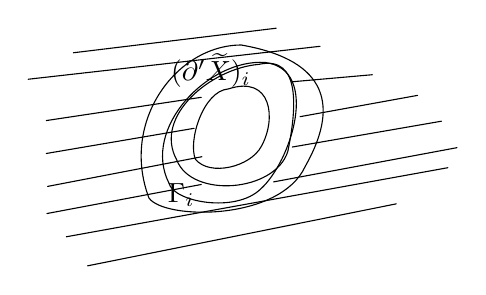
\begin{tikzpicture}[x=0.82cm,y=0.82cm,line cap=round]
\draw[thin] (-2.7,2.28)--(0.44,2.66) (-3.4,1.87)--(1.12,2.38)
 (-3.12,1.23)--(-0.72,1.59) (0.68,1.83)--(1.93,1.94)
 (-3.12,0.72)--(-0.83,1.11) (0.81,1.29)--(2.63,1.62)
 (-3.10,0.21)--(-0.71,0.67) (0.69,0.82)--(3.00,1.22)
 (-3.11,-0.21)--(-0.72,0.24) (0.40,0.28)--(3.24,0.81)
 (-2.81,-0.57)--(3.10,0.50) (-2.48,-1.02)--(2.30,-0.06);
\draw (-1.53,0.03) .. controls (-1.98,1.22) and (-1.10,2.40) .. (-0.10,2.40)
 .. controls (1.10,2.19) and (1.49,1.58) .. (0.89,0.52)
 .. controls (0.50,-0.33) and (-1.29,-0.31) .. cycle;
\draw (-1.22,0.26) .. controls (-1.65,1.11) and (-0.61,2.19) .. (0.27,2.13)
 .. controls (1.13,2.02) and (0.67,0.59) .. (0.20,0.17)
 .. controls (-0.19,-0.21) and (-1.15,-0.03) .. cycle;
\draw (-1.10,0.62) .. controls (-1.47,1.30) and (-0.56,2.04) .. (0.17,2.10)
 .. controls (0.84,2.25) and (0.75,1.38) .. (0.62,0.75)
 .. controls (0.42,0.12) and (-0.87,0.02) .. cycle;
\draw (-0.81,0.63) .. controls (-0.93,0.91) and (-0.69,1.69) .. (-0.30,1.72)
 .. controls (0.37,1.94) and (0.45,1.26) .. (0.21,0.83)
 .. controls (0.04,0.51) and (-0.59,0.36) .. cycle;
\node at (-0.57,2.00) {$ (\partial'\widetilde X)_i $};
\node at (-1.03,0.08) {$\Gamma_i$};
\end{tikzpicture}}
% slanted
\margin{C'est une composition rétrécissage $\circ$ élargissage, ou mieux élargissage $\circ$ rétrécissage.}

\unsure{4°)|4 bis)|5°)|4')} \uline{Commutation} de l'opération de panachage relative à diverses composantes connexes de $K$.

6) Cas d'une composante \inserted{$C$} de $K$ boucle isolée \inserted{plongée $\mathbb R$-analytique}. L'opération de panachage revient alors tjrs à une composition de 1) enlever une couronne \inserted{$\mathbb R$-analytique} autour de $C$ 2°) Recoller \inserted{$\mathbb R$-analytiq\textsuperscript{mt}} par un cylindre les deux bords \inserted{\unsure{qui restent|jointifs|joints}} de la couronne enlevée....

\figure{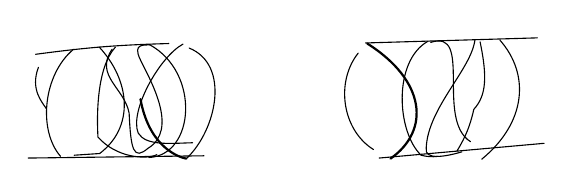
\begin{tikzpicture}[x=0.72cm,y=0.72cm,line cap=round]
\draw (0,0)--(3.1,0.04) (0.13,1.83) to[bend left=3] (2.48,2.02);
\draw (0.80,1.92) .. controls (0.26,1.47) and (0.17,0.49) .. (0.57,0.03);
\draw[thin] (0.18,1.60) .. controls (0.03,1.21) and (0.25,0.98) .. (0.32,0.87);
\draw (1.54,1.96) .. controls (1.20,1.59) and (1.21,0.72) .. (1.23,0.37) .. controls (1.56,0) and (2.08,-0.03) .. (2.27,0.06);
\draw[thin] (1.25,1.96) .. controls (1.80,1.37) and (1.88,0.55) .. (1.26,0.08)--(0.81,0.05);
\draw (1.48,1.92) .. controls (1.16,1.45) and (1.70,1.24) .. (1.78,0.79) .. controls (1.81,0.13) and (1.86,-0.04) .. (2.11,0.17)
 .. controls (2.66,0.50) and (2.16,1.36) .. (1.98,1.73) .. controls (1.82,2.05) and (2.08,1.98) .. (2.15,2.00);
\draw (2.14,2.0) .. controls (3.04,1.51) and (2.94,0.05) .. (2.13,0.01);
\draw (2.73,2.01) .. controls (2.32,1.79) and (1.78,0.83) .. (1.94,0.44) .. controls (2.08,0.21) and (2.50,0.26) .. (2.90,0.27);
\draw[thick] (1.98,1.04) .. controls (2.12,0.26) and (2.58,0.03) .. (2.79,-0.01);
\draw (2.84,1.94) .. controls (3.57,1.64) and (3.32,0.50) .. (2.80,0.00);
\begin{scope}[shift={(5.9,0)}]
\draw (0.05,2.03)--(3.08,2.12) (0.29,0.00)--(3.20,0.26);
\draw[thin] (-0.08,1.85) .. controls (-0.48,1.35) and (-0.37,0.50) .. (0.19,0.15);
\draw[thick] (0.08,2.02) .. controls (1.11,1.37) and (1.20,0.49) .. (0.49,-0.01);
\draw (1.15,2.06) .. controls (0.53,1.71) and (0.60,0.46) .. (1.03,0.05) to[bend right=10] (1.33,0.03);
\draw[thin] (1.20,2.04) .. controls (1.95,2.29) and (1.28,0.68) .. (1.90,0.29);
\draw (1.98,2.09) .. controls (1.92,1.57) and (1.15,0.89) .. (1.12,0.18) .. controls (1.08,-0.05) and (1.48,0.03) .. (1.75,0.11);
\draw (2.07,2.05) .. controls (2.20,1.43) and (2.18,1.10) .. (1.96,0.86) to[bend left=9] (1.66,0.12);
\draw[thin] (2.42,2.08) .. controls (2.95,1.48) and (2.89,0.63) .. (2.10,-0.02);
\end{scope}
\end{tikzpicture}}

\deleted{\figure{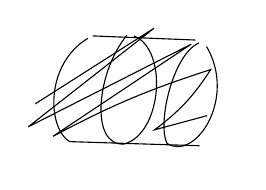
\begin{tikzpicture}[x=0.75cm,y=0.75cm]
\draw (0.37,1.66) .. controls (-0.37,1.21) and (-0.31,0.13) .. (0.06,-0.09) -- (2.26,-0.16);
\draw (0.45,1.70)--(2.19,1.63);
\draw (1.03,1.71) .. controls (0.51,1.08) and (0.40,-0.18) .. (0.99,-0.13) .. controls (1.63,0.06) and (1.73,1.47) .. (1.15,1.70);
\draw (2.25,1.58) .. controls (1.81,1.39) and (1.54,0.22) .. (1.71,-0.12) .. controls (2.18,-0.43) and (2.90,0.63) .. (2.38,1.52);
\draw (-0.52,0.55)--(1.49,1.83)--(-0.64,0.16)--(2.12,1.56)--(-0.22,0.00) to[bend left=5] (2.45,1.13) to[bend right=-10] (1.50,0.11)--(2.39,0.35);
\end{tikzpicture}}}

relations avec les \deleted{\unsure{deux|de}} \inserted{petits} \unsure{plong\textsuperscript{mts}|plongements|plongés} conformes d'une petite couronne...

% archive sheet number: 3
